%license:BSD-3-Clause
%copyright-holders:Michele Maione
%============================================================
%
%	Piattaforma di cloud gaming per giochi arcade
%
%============================================================

\chapter{Architettura del sistema}
%In questa sezione si deve descrivere l’obiettivo della ricerca, le problematiche affrontate ed eventuali definizioni preliminari nel caso la tesi sia di carattere teorico.
%In questa sezione si spiega come è stato affrontato il problema concettualmente, la soluzione logica che ne è seguita senza la documentazione.
In questo capitolo verrà descritto il sistema proposto, il MAME e le sue funzioni di: rendering, missaggio audio e gestione dell'input utente.



\section{Sistema proposto}
L'esigenza per la quale nasce questo progetto è far conoscere alle nuove generazioni i videogiochi che hanno fatto la storia e dare la possibilità di poter giocare ancora a macchine che ormai hanno cessato di funzionare per motivi di obsolescenza, sfruttando due tecnologie entrate a far parte della quotidianità, lo streaming e il cloud computing. In questo lavoro si propone la creazione di una piattaforma di cloud gaming, che permette lo streaming audio-video direttamente e su richiesta dei videogiochi, da un server remoto, ad un client (computer, console, telefono). Per far ciò verrà ampliato il software MAME\footnote{In seguito chiamato MAME CGP (Cloud Gaming Platform).} (rilasciato sotto licenza GNU-GPL) che è in grado di emulare oltre 7.000 giochi arcade. Le caratteristiche principali del progetto, che sono state vincolanti nella scelta delle tecnologie da utilizzare, sono la portabilità e la possibilità di utilizzare il sistema senza dover installare software aggiuntivi, e per questi vincoli, lato client, la scelta è ricaduta sul browser web.

Il sistema è stato progettato con un'ottica incentrata sull'utilizzo in LAN con l'utenza connessa tramite WiFi, ad esempio in stand di retro-gaming ad eventi di informatica e videogiochi, in aziende come servizio di svago per i clienti in sala d'attesa e per i dipendenti durante la pausa, ecc\dots. La tecnologia di streaming scelta è stata WebSocket per i seguenti motivi: in questo contesto la differenza di velocità tra TCP e RTP può essere trascurata, è un protocollo di comunicazione standardizzato dal 2011, è pienamente supportato da tutti i browser moderni, ha una latenza inferiore rispetto ad HLS e DASH, è semplice da instanziare e non richiede l'utilizzo di protocolli aggiuntivi o configurazioni complesse a differenza di WebRTC.

Come mostrato in Fig. \ref{fig:proposed_system} il sistema è costituito dal server di gioco (Linux, Windows o macOS), su cui è installato il MAME CGP con le rom dei giochi ed una pagina HTML5 che funge da front-end. Il programma è in ascolto per connessioni WebSocket con parametri (per es.: il nome del gioco, l'ID del player, l'ID della partita, ecc\dots). Una volta stabilita la connessione, il server invia informazioni sulla risoluzione di rendering e avvia il gioco. Il rendering e il missaggio audio del gioco vengono generati utilizzando la libreria SDL\footnote{SDL: Simple DirectMedia Layer, una libreria multipiattaforma ed open-soure per il multimedia.}, codificati e pacchettizzati nel contenitore MPEG-TS\footnote{MPEG-TS: MPEG transport stream, è un contenitore digitale per la trasmissione e l'archiviazione audio-video.} usando la libreria FFmpeg\footnote{FFmpeg è una suite open-source di librerie e programmi per la gestione di video, audio, e altri file multimediali e stream.} e inviati tramite WebSocket al client.

\begin{figure}[H]
	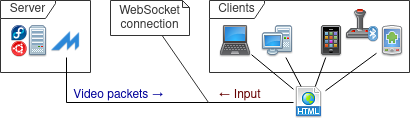
\includegraphics[width=\linewidth]{immagini/proposed_system}
	\caption{Panoramica del sistema}
	\label{fig:proposed_system}
\end{figure}

Lato client vari script si occupano di: decodificare i dati audio-video ricevuti, catturare e inviare l'input dell'utente (sia dalla tastiera che dal gamepad) al server tramite WebSocket.

\section{MAME}
Multiple Arcade Machine Emulator (MAME) è un progetto open-source (GNU-GPL) di Nicola Salmoria. La prima versione del MAME risale al febbraio 1997 ed è attualmente supportato da una vasta comunità di sviluppatori da tutto il mondo. Lo scopo principale è quello di essere un riferimento al funzionamento interno delle macchine emulate, sia per scopi educativi che per scopi di conservazione, al fine di evitare che il software storico scompaia per motivi di obsolescenza. Il progetto è stato realizzato in C++, inizialmente usando solamente la libreria standard e poi successivamente, negli anni, sono state aggiunte al progetto varie librerie open-source per estenderne le funzionalità. Originariamente era disponibile solo per MS-DOS ma grazie alla vasta comunità di sviluppatori è stato portato per i sistemi Windows e Unix-like\cite{MAME}.

\begin{figure}[H]
	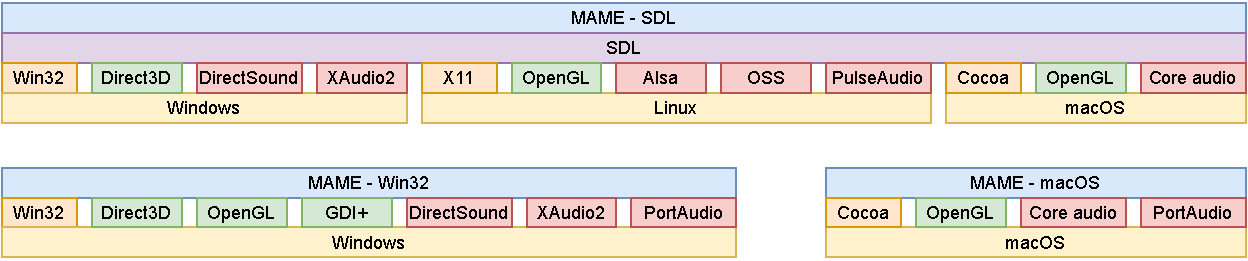
\includegraphics[width=\linewidth]{immagini/mame_architettura_full}
	\caption{MAME livelli di astrazione su diverse piattaforme}
	\label{fig:mame_architettura_full}
\end{figure}

Per quanto riguarda la portabilità, di cui c'è uno schema in Fig. \ref{fig:mame_architettura_full}, ci sono solo tre compilazioni native differenti e sono quella per macOS, Windows ed UWP\footnote{UWP - Universal Windows Platform è un'architettura applicativa della Microsoft per sviluppare applicazioni eseguibili su Windows 10, Xbox One e Hololens.}, in aggiunta c'è la compilazione che deriva da un port del MAME, il progetto SDLMAME\footnote{SDLMAME era un fork del MAME che utilizzava solamente la libreria SDL. Nel 2010 è stato incluso ufficialmente nel progetto MAME.} in grado di funzionare su tutti i sistemi operativi supportati dalla libreria SDL. Quest'ultima è la compilazione obbligatoria per i sistemi Linux e per questo motivo è quella che si è scelta di utilizzare per questo server di cloud gaming.

Simple DirectMedia Layer (SDL) è una libreria multipiattaforma che fornisce accesso di basso livello ad audio, tastiera, mouse, gamepad, hardware 3D e framebuffer 2D. Come mostrato in Fig. \ref{fig:mame_architettura_full} nello schema in alto, SDL è costruito sopra le API di visualizzazione video del sistema operativo (in arancione), librerie di rendering 3D (in verde) e librerie che si interfacciano alla scheda audio (in rosso)\cite{SDL_Wiki}. 

MAME, alla versione attuale (v. 0.228), è formato da 14.904 file sorgenti (e nel conteggio non ci sono i file di definizione della UI, gli script per la compilazione e le librerie esterne che sono incluse nel progetto sotto forma di sorgenti) ed è suddiviso in quattro macro categorie, come mostrato in Fig. \ref{fig:mame_arch}, che sono:

\begin{figure}[H]
	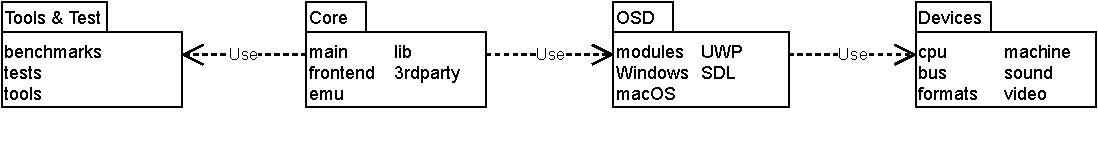
\includegraphics[width=\linewidth]{immagini/mame_arch}
	\caption{MAME, diagramma dei packages}
	\label{fig:mame_arch}
\end{figure}

\begin{itemize}
	\item "Core" in cui ci sono i sotto-progetti indipendenti dal sistema e dal device emulato tra cui il programma main a linea di comando (progetto main), il front-end grafico, il motore di emulazione (progetto emu), alcune librerie comuni a tutto il software (lib) ed i sorgenti delle librerie esterne (3rdparty);
	\item "OSD" contenente le funzionalità sia dipendenti dal sistema operativo come macOS, Windows, UWP ed SDLMAME, sia i moduli (progetto modules) di input, audio e video dipendenti da altre librerie come OpenGL, DirectX, SDL, CoreAudio, XAudio, XInput, ecc\dots;
	\item "Devices" che contiene per ogni device emulato (ad esempio il Capcom CP System III) le classi che gestiscono le informazioni della macchina ed emulano cpu, bus, video, audio e i dischi (progetto formats);
	\item "Tools \& Test" che contiene varie utility per la gestione delle rom e per la fase di testing (progetti benchmarks, tests, tools).
\end{itemize}



\subsection{Rendering}
Il MAME è in grado di emulare giochi sia 2D che 3D (es.: Tekken della Namco), ma poiché emula fisicamente il monitor del cabinato ciò che viene inviato alla libreria grafica è un insieme di primitive e texture da disegnare.

\begin{figure}[H]
	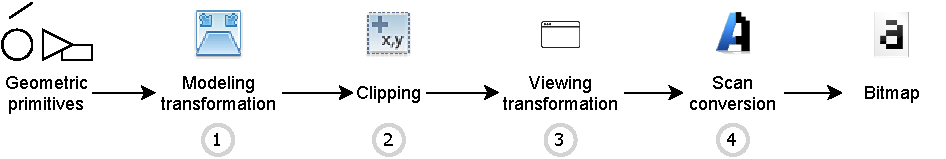
\includegraphics[width=\linewidth]{immagini/rendering_pipeline}
	\caption{Pipeline di rendering 2D}
	\label{fig:rendering_pipeline}
\end{figure}

Quando la finestra di gioco viene inizializzata, viene creato un contesto di rendering SDL per la finestra tramite la funzione \textit{CreateRenderer}. Per ogni frame della macchina che viene emulato c'è una fase di disegno usando \textit{SetRenderDrawColor}, \textit{RenderFillRect} e \textit{RenderDrawLine}, e poi tramite la funzione \textit{RenderPresent} viene mostrato il frame appena renderizzato sulla finestra.

In Fig. \ref{fig:mame_render_class_diagram} è visibile un diagramma delle classi relativo alla sola funzionalità di rendering (la controparte del missaggio audio funziona in maniera simile). È importante sottolineare che l'interfaccia grafica del MAME viene disegnata con le stesse procedure utilizzate per l'emulazione, e questo consente al nostro progetto di poter effettuare lo streaming anche dell'interfaccia grafica che può essere usato al posto del front-end HTML.

\begin{figure}[H]
	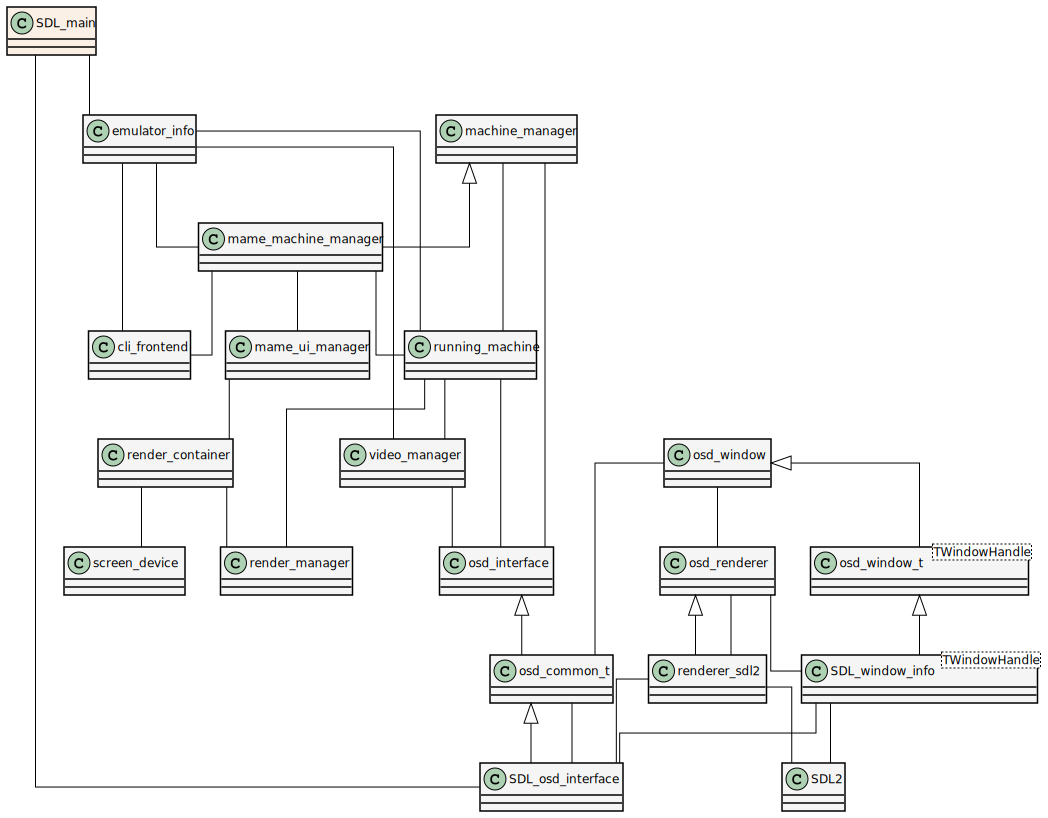
\includegraphics[width=\linewidth]{immagini/mame_render_class_diagram}
	\caption{MAME, diagramma delle classi relativo al rendering}
	\label{fig:mame_render_class_diagram}
\end{figure}



\subsection{Missaggio audio}
Lorem ipsum dolor sit amet, consectetur adipiscing elit, sed do eiusmod tempor incididunt ut labore et dolore magna aliqua. Ut enim ad minim veniam, quis nostrud exercitation ullamco laboris nisi ut aliquip ex ea commodo consequat. Duis aute irure dolor in reprehenderit in voluptate velit esse cillum dolore eu fugiat nulla pariatur. Excepteur sint occaecat cupidatat non proident, sunt in culpa qui officia deserunt mollit anim id est laborum.


\subsection{Gestione input}
Lorem ipsum dolor sit amet, consectetur adipiscing elit, sed do eiusmod tempor incididunt ut labore et dolore magna aliqua. Ut enim ad minim veniam, quis nostrud exercitation ullamco laboris nisi ut aliquip ex ea commodo consequat. Duis aute irure dolor in reprehenderit in voluptate velit esse cillum dolore eu fugiat nulla pariatur. Excepteur sint occaecat cupidatat non proident, sunt in culpa qui officia deserunt mollit anim id est laborum.
\cite{CPP_Primer}
\cite{Computer_Networking_and_the_Internet}
\cite{Ingegneria_del_software}
\cite{Understanding_the_Linux_Kernel}
\cite{Windows_Server_2012}